\documentclass{article}
\usepackage{packages}
\usepackage{macros}

\title{Progressing Domain Condition for Size-Change Termination and the Global Trace Condition with Injective Relations}
\author{Stefano Berardi}
\date{May, 2025}

\begin{document}

\maketitle

\section{Introduction}

\section{Size-change termination}
\textit{Size-change termination} (SCT), initially proposed by Lee et al. \cite{Lee1}, is a technique for proving the termination of recursive functions. SCT leverages Fermat's principle of infinite descent: to prove a proposition $P$, assume its negation and derive a contradiction by constructing an infinite descending chain within a well-ordered set. In the context of recursive functions, if the function's variables are interpreted within a well-ordered domain, non-termination can be assumed, and a contradiction derived by demonstrating an impossible infinite descending sequence of variable values. These sequences are formed by analyzing the relationships between variables across recursive calls. Each relationship is abstracted as a \textit{size-change graph}, which represents variable transformations during program execution. To make this concept precise, we begin by presenting some preliminary definitions, following the exposition in \cite{Lee1, Mirai}.

\begin{definition}
    \textbf{(Function names and parameters, \cite{Lee1, Mirai}):}
    For a program $P$, let $F$ be a finite set of \textit{function names} that appear in $P$, such that for each $f \in F$, we have $n$ distinct symbols $x_1^f,...,x_n^f$ named the \textit{parameters} of $f$, where the \textit{arity} of $f$ is defined as $arity(f) = n$. We define $Par(f) = \{x_1^f,...,x_n^f \}$ as the set of parameters of $f$.
\end{definition}

\begin{definition}
    \textbf{(Size-change graphs, \cite{Lee1, Mirai}):} Let $P$ be a program and $F$ the set of function names, and $f,g \in F$. A size-change graph from $f$ to $g$, written $G: f \rightarrow g$, is a bipartite graph defined as $G = (Par(f), Par(g), E)$, where $E \subseteq Par(f) \times \{ \downarrow, \downmapsto \} \times Par(g) $ and $E$ does not contain both $x_i^f \xrightarrow{\downarrow} x_j^g$ and $x_i^f \xrightarrow{\downmapsto} x_j^g$.  
\end{definition}

The edges $x_i^f \xrightarrow{\gamma} x_j^g$ represent the relationship between the values of the variables initially passed to the function, and the values passed in each recursive call. When $\gamma = \ \downarrow$, we call it a \textit{progressing} edge and it specifies that the value of $x_i^f$ is strictly less than the value of $x_j^g$. When $\gamma = \downmapsto$, we call it a \textit{weakly-progressing} edge, and it specifies that the value of $x_i^f$ is less than or equal to the value of $x_j^g$. To illustrate this concept, consider the following example of the Ackermann function, taken from \cite{Lee2}: 

\begin{example}
\label{ExampleSCT1}
For the program in Figure \ref{figFuncF}, we set $F = \{ ack\}$, with $arity(ack) = 2$. For each recursive call, labeled with 1,2 and 3, we can respectively define the size-change graphs $G_1$, $G_2$ and $G_3$. Note that even though the recursive calls 1 and 2 have different input values, their size-change graphs are exactly the same.


\begin{figure}[ht]
  \vspace{0.5cm}
  \centering
  % Minipage for the code listing
  \begin{minipage}[b]{0.45\textwidth}
    \begin{lstlisting}[basicstyle=\normalsize\ttfamily]
ack(m,n) = if m=0 then n+1 else
         if n=0 then *${}^{1}$*ack(m-1,1) else
         *${}^{2}$*ack(m-1,*${}^{3}$*ack(m,n-1))
    \end{lstlisting}
  \end{minipage}
  % Minipage for the first TikZ figure
  \begin{minipage}[b]{0.25\textwidth}
    \centering
    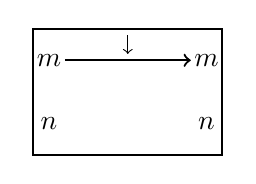
\begin{tikzpicture}[scale=0.8]
      % Draw the rectangle frame
      \draw[thick] (-1.5,-1.0) rectangle (1.5,1.0);
      % Place the nodes
      \node at (-1.25, 0.5) {$m$};
      \node at (1.25, 0.5) {$m$};
      \node at (-1.25, -0.5) {$n$};
      \node at (1.25, -0.5) {$n$};
      % Draw arrows m -> m
      \draw[thick, ->] (-1.0,0.5) -- (1.0,0.5);
      \draw[->] (0, 0.9) -- (0, 0.6);
    \end{tikzpicture}
    
    \vspace{0.1cm}
    
    $G_1, G_2$
  \end{minipage}
  % Minipage for the second TikZ figure
  \begin{minipage}[b]{0.25\textwidth}
    \centering
    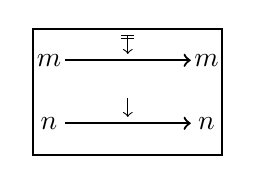
\begin{tikzpicture}[scale=0.8]
      % Draw the rectangle frame
      \draw[thick] (-1.5,-1.0) rectangle (1.5,1.0);
      % Place the nodes
      \node at (-1.25, 0.5) {$m$};
      \node at (1.25, 0.5) {$m$};
      \node at (-1.25, -0.5) {$n$};
      \node at (1.25, -0.5) {$n$};
      % Draw arrows m -> m
      \draw[thick, ->] (-1.0,0.5) -- (1.0,0.5);
      \draw (-0.1, 0.9) -- (0.1, 0.9);
      \draw (-0.1, 0.85) -- (0.1, 0.85);
      \draw[->] (0, 0.9) -- (0, 0.6);
      % Draw arrows n -> n
      \draw[thick, ->] (-1.0,-0.5) -- (1.0,-0.5);
      \draw[->] (0, -0.1) -- (0, -0.4);
    \end{tikzpicture}
    
    \vspace{0.1cm}
    
    $G_3$
  \end{minipage}
  \caption{Definition of the Ackermann function \texttt{a} and size-change graphs $G_1$, $G_2$ and $G_3$}
  \label{figFuncF}
\end{figure}
\end{example}

The termination behavior of a program $P$ can be inferred by examining the size-change graphs it induces. In particular, we study how these graphs compose to form \textit{multipaths}, as they reveals whether infinite descending chains (indicatives of termination) can occur.

\begin{definition}
    \textbf{(Composable graphs, \cite{Lee1, Mirai}):} Let $f,g,g',h, \in F$, with $G_1 = (Par(f), Par(g), E)$ and $G_2 = (Par(g'), Par(h), E')$ two size-change graphs. We say that $G_1$ and $G_2$ are \textit{composable}, if $g = g'$. We write $G_1G_2 = (Par(f)\cup Par(g) \cup Par(h), E \cup E')$ for the directed graph obtained by the union of $G_1$ and $G_2$.
\end{definition}

\begin{definition}
    \textbf{(Multipaths, threads and infinite descent\cite{Lee1, Mirai})} Let $\mathbb{G}$ be a set of size-change graphs: 
    \begin{enumerate}
        \item A \textit{$\mathbb{G}$-multipath} is a finite or infinite sequence $\mathcal{M} = G_1G_2...$ of size-change graphs in $\mathbb{G}$, such that for every $i$, $G_i$ and $G_{i+1}$ are composable. $\mathcal{M}$ can be viewed as a (possibly infinite) directed graph.
        
        \item A \textit{thread} in $\mathcal{M}$ is a (possibly infinite) directed path in $\mathcal{M}$. 
        
        \item We say that a thread is \textit{progressing} if it contains a progressing edge. Moreover, a thread is \textit{infinitely progressing} if it contains infinitely many progressing edges
        
        \item A multipath $\mathcal{M}$ has infinite descent if some thread thread in $\mathcal{M}$ is infinitely descending.
    \end{enumerate}  
\end{definition}

\begin{example}
\label{ExampleSCT2}
Suppose there is a hypothetical infinite execution starting from an initial call of the program \texttt{ack}, introduced in Example \ref{ExampleSCT1}. This execution is represented by the infinite sequence of recursive calls $c = 1313...$ or more compactly $(13)^{\omega}$. It induces the corresponding multipath $\mathcal{M} = G_1 G_3 G_1 G_3 ...$ as shown in Figure \ref{multipath}. Within this multipath, we can identify an infinitely progressing thread over the variable $m$, given by the sequence $m \xrightarrow{\downarrow} m \xrightarrow{\downmapsto} m \xrightarrow{\downarrow} m \ldots$.



\begin{figure}[h]
\vspace{0.5cm}
\centering
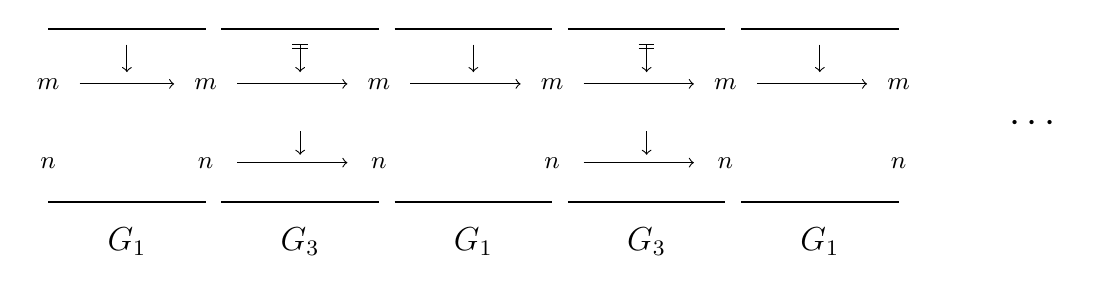
\begin{tikzpicture}[scale=1, every node/.style={font=\small}]

\def\xstep{2.2}

% BLOCK 1
\begin{scope}[xshift=0*\xstep cm]
  \node at (-1, 0.5) {$m$};
  \node at ( 1, 0.5) {$m$};
  \node at (-1,-0.5) {$n$};
  \node at ( 1,-0.5) {$n$};
  \draw[->] (-0.6, 0.5) -- (0.6, 0.5);
  \draw[->] (0, 1.0) -- (0, 0.65);
  
  \draw[thick, -] (-1, 1.2) -- (1, 1.2);
  \draw[thick, -] (-1, -1) -- (1, -1);
  \node at (0.0,-1.5) {\large $G_1$};
\end{scope}

% BLOCK 2 
\begin{scope}[xshift=1*\xstep cm]
  \node at ( 1, 0.5) {$m$};
  \node at ( 1,-0.5) {$n$};
  \draw[->] (-0.8, 0.5) -- (0.6, 0.5);
  \draw[->] (-0.8,-0.5) -- (0.6,-0.5);
  \draw[->] (0, 1.0) -- (0, 0.65); 
  \draw (-0.1,1.0) -- (0.1,1.0);   
  \draw (-0.1,0.95) -- (0.1,0.95);
  \draw[->] (0,-0.1) -- (0,-0.4);
  
  \draw[thick, -] (-1, 1.2) -- (1, 1.2);
  \draw[thick, -] (-1, -1) -- (1, -1);
  \node at (0.0,-1.5) {\large $G_3$};
\end{scope}

% BLOCK 3
\begin{scope}[xshift=2*\xstep cm]
  \node at ( 1, 0.5) {$m$};
  \node at ( 1,-0.5) {$n$};
  \draw[->] (-0.8, 0.5) -- (0.6, 0.5);
  \draw[->] (0, 1.0) -- (0, 0.65);

  \draw[thick, -] (-1, 1.2) -- (1, 1.2);
  \draw[thick, -] (-1, -1) -- (1, -1);
  \node at (0.0,-1.5) {\large $G_1$};
\end{scope}

% BLOCK 4 (double dash on m)
\begin{scope}[xshift=3*\xstep cm]
  \node at ( 1, 0.5) {$m$};
  \node at ( 1,-0.5) {$n$};
  \draw[->] (-0.8, 0.5) -- (0.6, 0.5);
  \draw[->] (-0.8,-0.5) -- (0.6,-0.5);
  \draw[->] (0, 1.0) -- (0, 0.65);
  \draw (-0.1,1.0) -- (0.1,1.0);
  \draw (-0.1,0.95) -- (0.1,0.95);
  \draw[->] (0,-0.1) -- (0,-0.4);

  \draw[thick, -] (-1, 1.2) -- (1, 1.2);
  \draw[thick, -] (-1, -1) -- (1, -1);
  \node at (0.0,-1.5) {\large $G_3$};
\end{scope}

% BLOCK 5
\begin{scope}[xshift=4*\xstep cm]
  \node at ( 1, 0.5) {$m$};
  \node at ( 1,-0.5) {$n$};
  \draw[->] (-0.8, 0.5) -- (0.6, 0.5);
  \draw[->] (0, 1.0) -- (0, 0.65);

  \draw[thick, -] (-1, 1.2) -- (1, 1.2);
  \draw[thick, -] (-1, -1) -- (1, -1);
  \node at (0.0,-1.5) {\large $G_1$};
\end{scope}



% BLOCK 6
\begin{scope}[xshift=5*\xstep cm]
  \node at ( 0.5, 0.0) {\Large$\cdots$};
\end{scope}

\end{tikzpicture}
\caption{Multipath generated by $(13)^{\omega}$}
\label{multipath}
\end{figure}

\end{example}

The underlying idea of SCT is that, by appealing to the principle of infinite descent, we can prove that a program $P$ terminates if every possible infinite execution would necessarily result in an infinite descending chain of variable values within a well-ordered domain. In other words, given a program $P$ and its associated set of size-change graphs $\mathbb{G}$, we observe that every infinite sequence of recursive calls $c$ in $P$, induces a corresponding multipath $\mathcal{M}$. If every such multipath exhibits infinite descent, then $P$ cannot have an infinite execution and must terminate. This observation leads to the formal definition of size-change termination condition:

\begin{definition}
    \textbf{(Size-change termination, \cite{Lee1, Mirai}):} Let $\mathbb{G}$ be a set of size-change graphs. We say that $\mathbb{G}$ satisfies the size-change termination (SCT) condition if every infinite $\mathbb{G}$-multipath has infinite descent.
\end{definition}




\section{Circular proof systems and the global trace condition}

The \textit{global trace condition} (GTC) is a criterion used to verify the validity of proofs in \textit{circular} and \textit{infinite proof systems}. In circular systems, proofs are represented as finite graphs with cycles, while in infinite systems, proofs take the form of infinite trees. Although the GTC admits different interpretations depending on the underlying proof system, a general abstraction can be formulated. In this work, we adopt a system-independent notion of the GTC, as presented by Brotherston \cite{brotherston} and further developed with a categorical framework by Afshari and Wehr \cite{Afshari_Wehr_2024}. In the case of latter, we consider the $\mathbb{B}$-activated trace category $\mathcal{T}_{\mathbb{B}}$, where $\mathbb{B} = \{\top, \bot\}$ is the binary boolean algebra. Although their framework provides a more general setting for describing trace conditions in circular proof systems, we will primarily rely on Brotherston's formulation to introduce the key concepts, for the sake of simplicity. Throughout this section, we focus exclusively on circular proof systems and do not consider infinite proof systems.

\subsection{Arbitrary circular proof systems}
An arbitrary \textit{circular proof system} $\text{CS}^{\omega}$ is given by a set of well-formed sequents $Seqs$, and a set of rules $Rules$, where each rule $R \in Rules$ is defined as:
\begin{figure}[H]
    \centering
    \begin{prooftree}
        \hypo{S_1 ...S_n}
        \infer1[$(R)$]{S}
    \end{prooftree}
\end{figure}
where $n \in \mathbb{N}$ and each $S_i$ and $S$ belong to $Seqs$. To formally represent the graph structure of a derivation in $\text{CS}^{\omega}$, we define the notions of a \textit{derivation graph} and a $\text{CS}^{\omega}$ \textit{pre-proof}.

\begin{definition}
    \textbf{(Derivation graph, \cite{brotherston}):} A $\text{CS}^{\omega}$ derivation graph, is a tuple $\mathcal{D} = (V, s, r, p)$ where:
    \begin{itemize}
        \item $V$ is a set of vertices
        \item $s: V \rightarrow Seqs$ is total function that labels vertices with sequents in $\text{CS}^{\omega}$
        \item $r: V \rightarrow Rules$ is partial function that labels vertices with inference rules in $S$
        \item $p: \mathbb{N} \times V \rightarrow V$ is a partial function that maps a number $n$ and a vertex $v$, with a vertex $v'$, such that $v'$ is labeled by the $n^{\text{th}}$ premise of the rule $r(v)$ over the sequent $s(v)$.
        \item For every $v \in V$, the following inference is an instance of the rule $r(v)$ in $S$, with $m$ premises:
            \begin{figure}[H]
                \centering
                \begin{prooftree}
                    \hypo{\{\vdash s(p(i,v))\}_{1 \leq i \leq m}}
                    \infer1[$(r(v))$]{\vdash s(v)}
                \end{prooftree}
            \end{figure}
    \end{itemize}

A derivation graph $\mathcal{D}$ is called a \textit{derivation tree} if its directed graph is a tree. Moreover, $\mathcal{D}$ is \textit{finite} (resp. \textit{infinite}) if the cardinality of $V$ is finite (resp. infinite). We say that $S$ is the \textit{endsequent} of a derivation tree $\mathcal{D}$, if the root node of the tree is labeled by $S$. A vertex $B \in V$ such that $r(B)$ is undefined. The set of bud nodes of a derivation graph $\mathcal{D}$, is written as $Bud(\mathcal{D})$.
\end{definition}


\begin{definition}
    \textbf{(Circular pre-proof, \cite{brotherston}):} A $\text{CS}^{\omega}$ pre-proof of a sequent $S$, is represented by a tuple $\mathcal{P} = (\mathcal{D}, \mathcal{R})$, where $\mathcal{D}$, is a $\text{CS}^{\omega}$ finite derivation tree with endsequent $S$, and $\mathcal{R}: V \rightarrow V$ is a partial function, that maps each one of the bud nodes in $Bud(\mathcal{D})$ to an internal node in the derivation tree, called a \textit{companion}, satisfying that if $B \in Bud(\mathcal{D})$ and $\mathcal{R}(B) = C$, then $r(C)$ is defined and $s(B) = s(C)$. We define the set of bud nodes of $\mathcal{D}$, as $Com(\mathcal{D})$.
\end{definition}

The combination of both the derivation tree $\mathcal{D}$ and the map $\mathcal{R}$ of a pre-proof $\mathcal{P}$, form a graph that can contain cycles. We call this graph $\mathcal{G}_{\mathcal{P}}$, and it is formally defined as:

\begin{definition}
    \textbf{(Pre-proof graph, \cite{brotherston}):} Let $\mathcal{P} = (\mathcal{D} = (V, s, r, p), \mathcal{R})$ be a $\text{CS}^{\omega}$ pre-proof. The graph of $\mathcal{P}$, written as $\mathcal{G}_{\mathcal{P}}$, is defined as $\mathcal{G}_{\mathcal{P}} = (V', s, r, p')$ where:
    \begin{itemize}
        \item $V' = V \setminus Bud(\mathcal{D})$
        \item $p'$ is defined as:
        \begin{align*}
            p'_j(v) \simeq 
            \begin{cases} 
                \mathcal{R}(p_j(v)) & \text{if $p_j(v) \in Bud(\mathcal{D})$} \\
                p_j(v) & \text{otherwise}
            \end{cases}
        \end{align*}
    for some $j \in \mathbb{N}$. We write $\simeq$ to say that $p'_j(v)$ is defined iff $\mathcal{R}(p_j(v))$ or $p_j(v)$ are defined, depending on the case. 
    \end{itemize}
    A pre-proof graph $\mathcal{G}_{\mathcal{P}}$ can be seen as a directed graph $(V', E)$ where the set of edges is defined as $E = \{(v, p'_j(v)) \ | \ v \in V \ \text{and $p'_j(v)$ is defined} \}$. A \textit{path} in $\mathcal{G}_{\mathcal{P}}$ is a finite or infinite sequence of vertices $v_0j_0v_1j_1v_2j_2...$ such that for all $i \geq 0$, $v_i \in V$, $j_i \in \mathbb{N}$ and $v_{i+1} = p'_{j_i}(v_{i})$. Sometimes, we will also write only $v_0v_1v_2...$ to specify a path without the succesor indexes.
\end{definition}

\begin{example}
\label{exampleCircProof}
We will use an example of a circular pre-proof in the $\text{CLKID}^{\omega}$ proof system, taken from \cite{brotherston}, to illustrate the previous definitions. In this system, inductive predicates are allowed, and we assume that the domain of the variables is $\mathbb{N}$ (or any other standard model of arithmetic). Each natural number is represented inductively, either as $0$ or using the successor function $s$. The rules for the inductive predicates $N$, $P$, and $Q$ are defined in Figure \ref{indRules}. Here, $P$ and $Q$ are mutually dependent inductive predicates, while $N$ corresponds to the standard inductive definition of the natural numbers.


\begin{figure}[h]
    \centering
\begin{minipage}{0.45\textwidth}
\centering
\begin{prooftree}
    \centering
    \hypo{}
    \infer1[($P\text{R}_1$)]{\Gamma \vdash P0, \Delta}
\end{prooftree}    
\end{minipage}
\hfill
\begin{minipage}{0.5\textwidth}
    \centering
    \begin{prooftree}
    \hypo{\Gamma \vdash Px, \Delta}
    \hypo{\Gamma \vdash Q(x,sx), \Delta}
    \infer2[($P\text{R}_2$)]{\Gamma \vdash Psx, \Delta}
\end{prooftree}
\end{minipage}

\vspace{0.3cm}

\begin{minipage}{.45\textwidth}
    \centering
    \begin{prooftree}
    \hypo{}
    \infer1[($Q\text{R}_1$)]{\Gamma \vdash Q(x,0), \Delta}
    \end{prooftree}
\end{minipage}
\hfill
\begin{minipage}{0.5\textwidth}
    \centering
    \begin{prooftree}
    \hypo{\Gamma \vdash Q(x,y), \Delta}
    \hypo{\Gamma \vdash Px, \Delta}
    \infer2[($Q\text{R}_2$)]{\Gamma \vdash Q(x,sy), \Delta}
\end{prooftree}
\end{minipage}

\begin{center}
\begin{prooftree}
    \hypo{\Gamma, x = 0 \vdash \Delta}
    \hypo{\Gamma, x = sz, Nz \vdash \Delta}
    \infer2[(Case $N$)]{\Gamma, Nx \vdash \Delta}
\end{prooftree}    
\end{center}

\caption{Rules in $\text{CLKID}^{\omega}$, for the unary predicates $N, P$ and the binary predicate $Q$}
\label{indRules}
\end{figure}

Figure \ref{circPreProof} presents an example of a circular pre-proof in the $\text{CLKID}^{\omega}$ proof system, which uses the rules defined for the inductive predicates $P$, $Q$, and $N$, along with standard structural rules such as contraction and weakening, as well as rules associated with first-order proof systems, such as equality substitution and variable renaming. The derivation graph corresponds to the tree structure shown in Figure \ref{circPreProof}, where the bud nodes are the leaves that have no rule associated with them, e.g. the leaves labeled with the sequent $Nx, Ny \vdash Q(x,y)$. The function $\mathcal{R}$ is represented by labeling each bud and its corresponding companion node with the same symbol, for example, the buds labeled $(\dag_1)$ and $(\dag_2)$ map to the companion labeled $(\dag)$, and similarly for the vertices labeled with $(*)$. The graph $\mathcal{G}_{\mathcal{P}}$ is then obtained by adding the edges induced by $\mathcal{R}$ and deleting the bud vertices from Figure \ref{circPreProof}.


\begin{figure}[h]
\centering
\begin{adjustbox}{scale=0.75}
\begin{prooftree}
        \hypo{}
        \infer1[($Q\text{R}_1$)]{Nx \vdash Q(x,0)}
        \infer1[($=$L)]{Nx, y=0 \vdash Q(x,y)}

        \hypo{Nx, Ny \vdash Q(x,y) \ (\dag_1)}
        \infer1[(Subst)]{Nx, Nz \vdash Q(x,z)}
        
        \hypo{}
        \infer1[$P\text{R}_1$]{\vdash P0}
        \infer1[(=L)]{x = 0 \vdash Px}
    
        \hypo{Nx \vdash Px \  (*)}
        \infer1[(Subst)]{Nz \vdash Pz}
        
        \hypo{Ny, Nx \vdash Q(x,y) \ (\dag_2)}
        \infer1[(Subst)]{Nsz, Nz \vdash Q(z, sz)}
        \infer[double]2[($P\text{R}_2$)]{Nsz, Nz \vdash Psz}
        \infer1[($=$L)]{Nx, x = sz, Nz \vdash Px}
        \infer[double]2[(Case $N$)]{Nx, Nx \vdash Px}
        \infer1[(Contr L)]{Nx \vdash Px \ (*)}
        \infer[double]2[($Q\text{R}_2$)]{Nx, Nz \vdash Q(x,sz)}
        \infer1[($=$L)]{Nx, y = sz, Nz \vdash Q(x,y)}   
        \infer2[(Case $N$)]{Nx, Ny \vdash Q(x,y) \ (\dag)}
\end{prooftree}
\end{adjustbox}

\caption{Example of a circular proof in $\text{CLKID}^{\omega}$ of the sequent $Nx, Ny \vdash Q(x,y)$. The double horizontal lines in some of the rules represent a hidden weakening rule.}
\label{circPreProof}
\end{figure}
\end{example}


\subsection{Generalized GTC}

In most circular proof systems, the validity or soundness of circular pre-proofs is expressed via the global trace condition (GTC). This condition can be generally stated as follows: ``A $\text{CS}^{\omega}$ pre-proof $\mathcal{P}$ satisfies the global trace condition, in which case we call it a $\text{CS}^{\omega}$ proof, if and only if every infinite path in $\mathcal{G}_{\mathcal{P}}$ has a \textit{trace} that \textit{infinitely progresses}.'' However, both the notion of a ``trace'' and what it means to ``infinitely progressing'' are defined differently depending on the circular proof system under consideration. Moreover, the \textit{semantic interpretation} of the GTC, which provides the soundness criterion for each system, also varies based on the specific characteristics of the circular proof system. For these reasons, we will devote the remainder of this section to presenting a generalized version of these concepts.

First, we introduce an abstract notion of semantics for a circular proof system. Given a circular proof system $\text{CS}^{\omega}$, we define $\mathbb{I}$ as a set of \textit{interpretations}, and write $I \models S$ to mean that the sequent $S$ is satisfied by the interpretation $I \in \mathbb{I}$. Moreover, a sequent $S$ is said to be \textit{valid} if it is satisfied by every interpretation $I \in \mathbb{I}$. The definition of each individual interpretation $I$ depends on the characteristics of the proof system. For example, a circular proof system involving predicates and first-order quantification, like $\text{CLKID}^{\omega}$ \cite{brotherston}, may be interpreted by a first-order structure $\mathcal{M}$ together with an environment $\rho$, whereas other systems such as the $\mu$-calculus \textcolor{red}{[CITATIONS]} use only an environment for the interpretation of the variables of a sequent over a particular domain. Therefore, to define the general notion of a trace, we introduce a \textit{trace function}:


\begin{definition}
\label{defTrace}
    \textbf{(Trace function \& trace, \cite{brotherston}):} Let $\mathcal{T}$ be a set, $\text{CS}^{\omega}$ a circular proof system, and $TVal \subseteq \mathcal{T} \times Seqs$ a relation satisfying that for all $S \in Seqs$, there are finitely many $\uptau \in \mathcal{T}$ such that $TVal(\uptau, S)$, and we define $TVal_S = \{\uptau \ | \ TVal(\uptau, S) \}$. Moreover, let $TPair: (\mathcal{T} \times \mathcal{T}) \rightarrow (Seqs \times Rules \times Seqs) \rightarrow \{0,1,2\}$ be a computable function satisfying:
    \begin{align*}
        \forall \uptau, \uptau', s, r, s'. \neg TVal(\uptau, s) \lor \neg TVal(\uptau', s') \Rightarrow TPair(\uptau , \uptau')(s, r, s') = 0
    \end{align*}
    Also, suppose there exists a function $\sigma : \mathcal{T} \times \mathbb{I} \rightarrow O$, where $O$ is some is initial segment of the ordinals satisfying that for any $\text{CS}^{\omega}$ pre-proof $\mathcal{P}$ with a graph $\mathcal{G}_{\mathcal{P}} = (V, s, r, p)$ then:
    \begin{align*}
        I \nvDash s(v) &\Rightarrow \exists I', v',j. \  v'= p_j(v) \\
        & \text{and} \ I' \nvDash s(v') \\
        & \text{and} \ TPair(\uptau, \uptau')(s(v), r(v), s(v')) = 1 \Rightarrow \sigma(\uptau', I') \leq \sigma(\uptau, I) \\
        & \text{and} \ TPair(\uptau, \uptau')(s(v), r(v), s(v')) = 2 \Rightarrow \sigma(\uptau', I') < \sigma(\uptau, I) \tag{1}
    \end{align*}
$TVal$ is called a \textit{trace value relation} and $TPair$ is called a \textit{trace pair function} for the proof system, and $\sigma$ is the \textit{ordinal trace function} associated with $TPair$ and $TVal$. The pair $(\uptau, \uptau')$ is said to be a \textit{valid trace pair} on $(v,v')$ if $TPair(\uptau, \uptau')(s(v), r(v), s(v')) \neq 0$, a \textit{weakly-progressing trace pair} on $(v,v')$ if $TPair(\uptau, \uptau')(s(v), r(v), s(v')) = 1$, and a \textit{progressing trace pair} on $(v,v')$ if $TPair(\uptau, \uptau')(s(v), r(v), s(v')) = 2$. Moreover, a sequence $(\uptau_i)$ of elements in $\mathcal{T}$ is a \textit{trace} on a path $(v_i)$, if for all $i$, $(\uptau_i,\uptau_{i+1})$ is a valid trace pair on $(v_i, v_{i+1})$. A trace $(\uptau_i)$ is said to \textit{progress} at $j$ if $(\uptau_j, \uptau_{j+1})$ is a progressing trace pair, and is said to be \textit{infinitely progressing} if there are infinitely many points at which it progresses.
\end{definition}

\begin{example}
To understand the intuition behind the previous definitions, we use the Example \ref{exampleCircProof}. In the case of the $\text{CLKID}^{\omega}$ circular proof system, as stated earlier, an interpretation $I$ for a sequent $\Gamma \vdash \Delta$ is given by the structure $\mathbb{N}$ together with an environment $\rho$ for the values of the variables, written as $\mathbb{N} \models_{\rho} \Gamma \vdash \Delta$. The relation $TVal$ associates inductive predicates $P(\vec{x})$ with sequents, meaning that if $P(\vec{x})$ is a formula occurring in the sequent $S$, then $TVal(P(\vec{x}), S)$ holds. The function $TPair$ describes how inductive predicates transform after the application of each rule in the proof system. For example, consider the first instance of the rule (Case $N$), with $v$ the root node, and $v_l$ and $v_r$ its left and right child nodes, respectively. Then, $TPair(Nx, Nx)(s(v), r(v), s(v_l)) = 1$, since the value of the variable $x$ remains unchanged after the application of the rule, and $TPair(Ny, Nz)(s(v), r(v), s(v_r)) = 2$, since the value of the variable $y$ is strictly decreased after the application of the rule.

The function $\sigma$ is defined as follows: given an interpretation $I = (\mathbb{N}, \rho)$ and the inductive predicate $Nx$, we have $\sigma(Nx, I) = \rho(x)$. In the case where the inductive predicate involves $n$ variables, we use the valuation $\rho(\vec{x}) = (\rho(x_1), \dots, \rho(x_n))$ and apply the lexicographical order. Then, the trace $\uptau = (Ny, Nz, Nz, Nz, Ny)^{\omega}$ is infinitely progressing, since the pair $TPair(Ny, Nz)(s(v), r(v), s(v_r))$ is progressing. Moreover, this trace can be used to validate all the infinite paths contained in the cycle from $(\dag)$ to $(\dag_1)$.  
\end{example}
 
Having defined the notion of a trace, we can now formally define the generalized version of the GTC. With this notion of the GTC, Brotherston proved that the generalized GTC implies the soundness of proofs in infinitary proof systems, by relying in the infinite descent method and the condition (1) of the Definition \ref{defTrace}. Moreover, his proof also implies the soundness of $\text{CS}^{\omega}$ proofs, since circular proofs can be viewed as a susbset of infinite proofs.

\begin{definition}
    \textbf{(Generalized global trace condition, \cite{brotherston}):} An $\text{CS}^{\omega}$ pre-proof $\mathcal{P}$ is said to be an $\text{CS}^{\omega}$ \textit{proof} if, for every infinte path in $\mathcal{G}_{\mathcal{P}}$ there is an infinitely progressing trace following some tail of the path.  
\end{definition}

\begin{proposition}
    \label{PropGTC}
    \textbf{(Soundness of generalized circular proofs, \cite{brotherston}):} If there is a $\text{CS}^{\omega}$ proof of the sequent $S$, then $S$ is valid.
\end{proposition}

\begin{example}
    We do not include the full proof of Proposition \ref{PropGTC}, as it can be found in the original work by Brotherston \cite{brotherston}. Instead, we provide an informal explanation using Example \ref{exampleCircProof}. The goal is to justify that in the circular proof shown in Figure   \ref{circPreProof}, the sequent $Nx, Ny \vdash Q(x,y)$ is valid, i.e. that for any environment $\rho$, $\mathbb{N} \models_{\rho} Nx, Ny \vdash Q(x,y)$. For those branches of the proof ending in axiomatic rules, validity can be established directly by induction on the rules themselves. However, this approach does not work for branches whose leaves are bud nodes, as these branches are not well-founded. In such cases, validity is established using the method of infinite descent. 
    
    Suppose, for contradiction, that there exists an environment $\rho$ such that $\mathbb{N} \nvDash_{\rho} Nx, Ny \vdash Q(x,y)$. Consider the branch corresponding to the bud node labeled $(\dag_1)$. Since we know this path has an infinitely progressing trace, namely $\uptau = (Ny, Nz, Nz, Nz, Ny)^{\omega}$, the interpretation of this trace under $\rho$ would yield an infinite descending chain of natural numbers. But this is impossible in $\mathbb{N}$, and thus our assumption must be false. Therefore, $\mathbb{N} \models_{\rho} Nx, Ny \vdash Q(x,y)$. Since each infinite path in $\mathcal{G}_{\mathcal{P}}$ represents a derivation, we must find an infinitely progressing trace for each one in order to establish the validity of the entire circular proof. It is easy to see, that for the pre-proof in Figure \ref{circPreProof}, every infinite path has a infinitely progressing trace, hence it is a $\text{CLKID}^{\omega}$ proof.
\end{example}

\section{Equivalence between GTC and SCT}
It has long been part of the folklore that the GTC and the SCT principle are equivalent. However, to the best of the authors' knowledge, this equivalence has only been formally established in the work of Ikebuchi \cite{Mirai}, specifically for the $\text{CLKID}^{\omega}$ circular proof system. For this reason, the following section is based on her results, with adaptations to the setting of the generalized GTC introduced earlier. The main objective of this section is to shed light on the formal correspondence between the generalized global trace condition and size-change termination. 

The general idea is as follows: given a circular pre-proof $\mathcal{P} = (\mathcal{D}, \mathcal{R})$ with a set of companion nodes $Com(\mathcal{D}) = \{C_1, \ldots, C_n\}$, we associate each companion node $C_i$ with a function symbol in the size-change framework. The arity of this function is given by $|TVal_{s(C_i)}|$, that is, the number of values associated with the sequent $s(C_i)$. With this in mind, we are now ready to define the size-change graphs associated with a circular pre-proof.


\begin{definition}
    \textbf{(Size-change graphs of a circular pre-proof, \cite{Mirai}):} Let $\mathcal{P} = (\mathcal{D, \mathcal{R}})$ be a circular pre-proof in $\text{CS}^{\omega}$, with $Bud(\mathcal{D}) = \{B_1,...,B_n \}$ and $Com(\mathcal{D}) = \{C_1,...,C_m \}$. Now consider any $B_i \in Bud(\mathcal{D})$ and $C_j \in Com(\mathcal{D})$, such that $C_j$ is an ancestor of $B_i$, i.e. there is a path from $C_j$ to $B_i$ in $\mathcal{D}$. Then, we define the size-change graph $G_{C_j, \mathcal{R}(B_i)} = (TVal_{s(C_j)}, TVal_{s(\mathcal{R}(B_i))}, E)$, where $E$ is defined as:
    
    \begin{itemize}
        \item $G_{C_j, \mathcal{R}(B_i)}$ has an arc $\uptau^{C_j}_k \xrightarrow{\downarrow} \uptau^{\mathcal{R}(B_i)}_l$ iff there is a progressing trace from $\uptau_k \in TVal_{s(C_j)}$, to $\uptau_l \in TVal_{s(\mathcal{R}(B_i))}$.
        \item $G_{C_j, \mathcal{R}(B_i)}$ has an arc $\uptau^{C_j}_k \xrightarrow{\downmapsto} \uptau^{\mathcal{R}(B_i)}_l$ iff there is a non-progressing trace from $\uptau_k \in TVal_{s(C_j)}$, to $\uptau_l \in TVal_{s(\mathcal{R}(B_i))}$.    
    \end{itemize}

    We define $\mathbb{G}_{\mathcal{P}}$, as the set of all such size-change graphs in $\mathcal{P}$.
\end{definition}

The equivalence between the GTC and the SCT principle was formally established by Ikebuchi~\cite{Mirai} for the $\text{CLKID}^{\omega}$ circular proof system. We now restate this result in a generalized setting, applying it to abstract circular proof systems.


\begin{proposition}
    \label{PropEqualCond}
    \textbf{(GTC and SCT equivalence, \cite{Mirai}):} For any $\text{CS}^{\omega}$ proof $\mathcal{P}$, $\mathbb{G}_{\mathcal{P}}$ satisfies the SCT condition. Conversly, for any $\text{CS}^{\omega}$ pre-proof $\mathcal{P}$, if $\mathbb{G}_{\mathcal{P}}$ satisfies the SCT condition, then $\mathcal{P}$ is a proof.
\end{proposition}

This proposition can be proved using the original proof strategy given by Ikebuchi in \cite{Mirai}. While her result was presented in the specific context of $\text{CLKID}^{\omega}$, the underlying reasoning is sufficiently general to apply to arbitrary circular proof systems.

\begin{example}
    \textcolor{red}{(USE IKEBUCHI'S OR ANOTHER EXAMPLE, TO GIVE INTUITION BEHIND THE PROPOSITION)}
\end{example}

%----------------------------------------------------
%----------------------------------------------------
%----------------------------------------------------
%----------------------------------------------------
%----------------------------------------------------

\section{Abstract SCT/GTC and the progress domain condition:}

Given the equivalence between SCT and GTC established in Proposition \ref{PropEqualCond}, it becomes evident that both conditions share two key characteristics: (1) both can be formulated using size-change graphs, and (2) the composition of these graphs relies on an underlying structure. In the case of SCT, this structure arises from the control flow between function calls. For GTC, it is determined by the position of the companion nodes in the graph structure of circular pre-proofs. Motivated by these commonalities, we now introduce a unified abstraction that captures both SCT and GTC within a single formal definition. 

\subsection{Bi-colored relation transition graphs:}
Building on observation (1), we begin by abstracting size-change graphs as \emph{bi-colored relations} over a finite set of variables. which will allow for a uniform treatment of both SCT and GTC.

\begin{definition}
    \textbf{(Bi-colored relations and pair composition):} Let $X = \{x_1, ..., x_n\}$ be a finite set of variables. A bi-colored relation over $X$, is a pair $(S,P)$ such that $S, P \subseteq X \times X$ where $S_i \cap P_i = \emptyset$. For two variables $x,y \in X$, If $xSy$ (resp. $xPy$) we say that $x$ \textit{weakly progresses} (resp. \textit{progresses}) to $y$ in $(S, P)$. Moreover, we define the composition of two pairs $(S,P)$ and $(S',P')$ as:
    \begin{align*}
    (S, P)(S', P') &= (S'' \setminus P'',\; P'')
    \end{align*}
    where $S''$ and $P''$ are defined as:
    \begin{align*}
    S'' = S \circ S  \quad P'' = (S \circ P') \cup (P \circ S') \cup (P \circ P')
    \end{align*}
\end{definition}

To capture observation (2), we introduce a transition system whose edges are labeled by bi-colored relations, abstracting both the control flow between function calls in SCT and the proof structure in circular pre-proofs for GTC. This general notion provides a common foundation for the unified treatment of SCT and GTC.

\begin{definition}
    \textbf{(Bi-colored relation transition graph):} Let $\mathcal{B} = \{(S_1,P_1),...,(S_n,P_n) \}$ be a set of bi-colored relations. We define a \textit{bi-colored relation transition graph}, as a labeled transition system represented by the tuple $\mathcal{T} =(V, \mathcal{B}, E)$ where: $V$ is a finite non-empty set of vertices and $E \subseteq V \times \mathcal{B}\times V$ is a set of directed edges labeled by bi-colored relations in $\mathcal{B}$.   
\end{definition}

\begin{definition}
    \textbf{(Composable)}
\end{definition}

\begin{example}
    \textcolor{red}{[Include here an example (THE SAME AS FOR SECTION 4) of how the three defintions SCT <-> GTC <-> transition graph interact][Make basically a triangle where each corner is each representation and each edge is a biconditional <->]}
\end{example}



\subsection{sdas}




%BIBLIOGRAPHY:
\bibliographystyle{ieeetr}
\bibliography{references}

\end{document}


\begin{comment}
\begin{definition}
    \textbf{($\rho$-interpreted circular proof system):} Let $\text{CS}^{\omega}$ be a circular proof system interpreted by $\mathbb{I}$. We say that $\text{CS}^{\omega}$ is \textit{$\rho$-interpreted}, if all sequents $S$ in $\text{CS}^{\omega}$ have a set of variables, and for any interpretation $I$ in $\mathbb{I}$ such that $I \models S$, then $I$ contains an environment $\rho$ for the value of the variables in $S$. 
\end{definition}
\end{comment}

\begin{comment}
    With this in mind, we explain the general intuition behind the GTC and why it ensure the soundness of circular pre-proofs. Consider then any pre-proof $\mathcal{P}$ of a sequent $S$ in a circular proof system $\mathcal{\text{CS}^{\omega}}$ interpreted by a set of interpretations $\mathbb{I}$. Usually, to prove the soundness of well founded proof systems, i.e. proof systems where the derivation is represented by a finite tree, it is sufficient to prove the local soundness of every rule, and use induction to prove the soundness of all proofs. In the case of circular pre-proofs, even though we can apply the same method to prove the soundness of branches that end in axiom rules, for the braches that cycle back to internal nodes it is not possible since they are non-well founded. The principle that is used to verify the soundness of branches with cycles is Fermats principle of infinite descent: To prove a proposition $P$, we assume its negation $\neg P$ and form an infinite descending chain of values using $\neg P$ in a well-order, which is impossible and hence we conclude by contradiction $P$. 

The way this principle is applied for circular proofs consists of assuming that the sequent $S$ is not valid
\end{comment}

\begin{comment}
    \subsection{Arbitrary finite proof systems}
First we define the notion of an arbitrary \textit{finite proof system}. An arbitrary finite proof system $S$ is given by a set of well-formed sequents $Seqs$, and a set of rules $Rules$, where each rule $R \in Rules$ is defined as:
\begin{figure}[H]
    \centering
    \begin{prooftree}
        \hypo{\Gamma_1 \vdash \Delta_1...\Gamma_n \vdash \Delta_n}
        \infer1[$(R)$]{S}
    \end{prooftree}
\end{figure}
where $n \in \mathbb{N}$ and each $\Gamma_i \vdash \Delta_i$ and $S$ belong to $Seqs$. To formally represent the graph structure of a derivation in $S$, we define a \textit{derivation graph}. An $S$ derivation graph, is a tuple $\mathcal{D} = (V, s, r, p)$, where $V$ is a set of vertices, $s: V \rightarrow Seqs$ is total function that labels vertices with sequents in $S$, $r: V \rightarrow Rules$ is partial function that labels vertices with inference rules in $S$, and $p: \mathbb{N} \times V \rightarrow V$ is a partial function that maps a number $n$ and a vertex $v$, with a vertex $v'$, such that $v'$ is labeled by the $n$th premise rule $r(v)$ over the sequent $s(v)$. The idea then is that for every $v \in V$, the following inference is an instance of the rule $r(v)$ in $S$, with $m$ premises:

\begin{figure}[H]
    \centering
    \begin{prooftree}
        \hypo{\{\vdash s(p(i,v))\}_{1 \leq i \leq m}}
        \infer1[$(r(v))$]{\vdash s(v)}
    \end{prooftree}
\end{figure}

Moreover, a derivation graph $\mathcal{D}$ is called a \textit{derivation tree} if its directed graph is a tree. We say that $S$ is the \textit{endsequent} or \textit{conclusion} of a derivation tree $\mathcal{D}$, if the root node of the tree is labeled by $S$. Since $r$ is partial function, a \textit{bud} node of $\mathcal{D}$ is a vertex $B \in V$ such that $r(B)$ is undefined. The set of bud nodes of a derivation graph $\mathcal{D}$, is written as $Bud(\mathcal{D})$. We then say that a \textit{finite proof} in $S$ of a sequent $S$, is a \textit{finite derivation tree} (i.e. a derivation tree with finite vertices) where the endsequent is $S$ and $Bud(\mathcal{D}) = \emptyset$.
\end{comment}




\begin{comment}
In the case of a finite proof system $S$, proving its soundness comes down to proving that every rule in $S$ is locally sound and then use induction over the inductive structure of the derivation trees to prove the soundness of all proofs. However, in the case of a circular proof system $\text{CS}^{\omega}$ this is not the same case. The main issue is that pre-proofs in $\text{CS}^{\omega}$ are not always trees, since their structure allow to form cycles. For this reason, the inductive reasoning used to proof soundness in finite proof systems can only be used in branches of the pre-proof that end in axiomatic leaves, i.e. leaves that end with an axiom rule, but branches that end with bud nodes can not be validated in this way, since they are non-well founded. Therefore, the soundness of the non-well founded branches of pre-proofs in $\text{CS}^{\omega}$, depend on a special criteria known as the global trace condition. The main intuition behind the global trace condition, used to prove the validity of pre-proofs lies on the following key points:
\begin{enumerate}
    \item First, we assume that the domain of interpretation of our interpretations $I$, is well-ordered.
    \item We use Fermat's principle of infinite descent, to prove that all infinite paths  
\end{enumerate}


Note that we call $\mathcal{P}$ a pre-proof, since we have not ensured that it represents a sound argument. Of course, this notion of soundness is dependent of the interpretation and semantics of the proof system in question. For this reason, we will assume an abstract notion of interpretation. We then define $\mathbb{I}$ as a set of interpretations



witand we have a semantic notion of satisfaction between interpretations. 


In the case of a finite proof system $S$, we prove that the system is sound by proving the local soundness of the rules 

given that a the soundness of the system has already been proven, we can always ensure that any derivation tree $\mathcal{D}$ in $S$ must be sound. However, this is not the case for circular proof systems $\text{CS}^{\omega}$


To do this, we must first define the GTC for $\text{CS}^{\omega}$ pre-proofs. The GTC leverages Fermat's principle of infinite descent: constructing an infinite descending chain of elements within a well-ordered set entails a contradiction. In the context of circular proofs, we need to make sure that every infinite path that    
\end{comment}